\documentclass[11pt]{article}
\usepackage[margin=2.5cm]{geometry}
\usepackage{booktabs}
\usepackage{float}
\usepackage{graphicx}
\usepackage{caption}
\usepackage{xcolor}
\usepackage{hyperref}
\hypersetup{colorlinks=true,linkcolor=blue,urlcolor=blue}
\title{GRouNdScale Model Scaling Report \\ \large Parameter Sizes, GPU Memory and Step Times across HVG Configurations (\texttt{size-compute})}
\author{Auto-generated from \texttt{size-compute} run logs}
\date{\today}
\begin{document}
\maketitle

\section{Overview}
This report summarises results from 32 completed training runs of the Causal GAN pipeline with increasingly higher highly variable gene (HVG) counts, from 1,000 to 16,500 in steps of 500. Each run uses the same model architecture and training configuration (20 training steps for the causal controller, followed by 20 steps for the main causal GAN), differing only in the number of highly variable genes selected during preprocessing.

The 17000 HVG run(s) were incomplete or failed at the time this report was generated and are excluded from all tables and figures. In particular, the 17,000 HVG run encountered CUDA out-of-memory during generator initialization.

All included runs completed without CUDA out-of-memory errors. The largest included run (16,500 HVGs) reached a peak GPU memory of 79,719\,MiB, approaching the GPU's 80\,GB capacity.

\section{GRN Characteristics}
\begin{table}[H]
\centering
\caption{Causal graph statistics for each HVG configuration. The TF/Target ratio is the number of transcription factors divided by the number of target genes.}
\label{tab:grn}
\begin{tabular}{rrrrrrrr}
\toprule
HVGs & TFs & Target Genes & TF/Target Ratio (\%) & Imposed Edges & Possible Edges & Edge Density (\%) \\
\midrule
1,000 & 63 & 928 & 6.79 & 13,920 & 58,464 & 23.8 \\
1,500 & 89 & 1410 & 6.31 & 21,150 & 125,490 & 16.9 \\
2,000 & 127 & 1873 & 6.78 & 28,095 & 237,871 & 11.8 \\
2,500 & 161 & 2339 & 6.88 & 35,085 & 376,579 & 9.3 \\
3,000 & 202 & 2798 & 7.22 & 41,970 & 565,196 & 7.4 \\
3,500 & 237 & 3263 & 7.26 & 48,945 & 773,331 & 6.3 \\
4,000 & 287 & 3713 & 7.73 & 55,695 & 1,065,631 & 5.2 \\
4,500 & 324 & 4176 & 7.76 & 62,640 & 1,353,024 & 4.6 \\
5,000 & 370 & 4630 & 7.99 & 69,450 & 1,713,100 & 4.1 \\
5,500 & 414 & 5086 & 8.14 & 76,290 & 2,105,604 & 3.6 \\
6,000 & 464 & 5536 & 8.38 & 83,040 & 2,568,704 & 3.2 \\
6,500 & 506 & 5994 & 8.44 & 89,910 & 3,032,964 & 3.0 \\
7,000 & 555 & 6445 & 8.61 & 96,675 & 3,576,975 & 2.7 \\
7,500 & 599 & 6901 & 8.68 & 103,515 & 4,133,699 & 2.5 \\
8,000 & 639 & 7361 & 8.68 & 110,415 & 4,703,679 & 2.3 \\
8,500 & 685 & 7815 & 8.77 & 117,225 & 5,353,275 & 2.2 \\
9,000 & 733 & 8267 & 8.87 & 124,005 & 6,059,711 & 2.0 \\
9,500 & 774 & 8726 & 8.87 & 130,890 & 6,753,924 & 1.9 \\
10,000 & 817 & 9183 & 8.90 & 137,745 & 7,502,511 & 1.8 \\
10,500 & 851 & 9649 & 8.82 & 144,735 & 8,211,299 & 1.8 \\
11,000 & 887 & 10113 & 8.77 & 151,695 & 8,970,231 & 1.7 \\
11,500 & 918 & 10582 & 8.68 & 158,730 & 9,714,276 & 1.6 \\
12,000 & 949 & 11051 & 8.59 & 165,765 & 10,487,399 & 1.6 \\
12,500 & 974 & 11526 & 8.45 & 172,890 & 11,226,324 & 1.5 \\
13,000 & 1002 & 11998 & 8.35 & 179,970 & 12,021,996 & 1.5 \\
13,500 & 1027 & 12473 & 8.23 & 187,095 & 12,809,771 & 1.5 \\
14,000 & 1045 & 12955 & 8.07 & 194,325 & 13,537,975 & 1.4 \\
14,500 & 1064 & 13436 & 7.92 & 201,540 & 14,295,904 & 1.4 \\
15,000 & 1098 & 13902 & 7.90 & 208,530 & 15,264,396 & 1.4 \\
15,500 & 1118 & 14382 & 7.77 & 215,730 & 16,079,076 & 1.3 \\
16,000 & 1131 & 14869 & 7.61 & 223,035 & 16,816,839 & 1.3 \\
16,500 & 1146 & 15354 & 7.46 & 230,310 & 17,595,684 & 1.3 \\
\bottomrule
\end{tabular}
\end{table}

\section{Training Step Times}
\begin{table}[H]
\centering
\caption{Average time per training step for the causal controller (first training phase) and causal generator (second training phase), extracted from the final step log line of each phase.}
\label{tab:step-times}
\begin{tabular}{rcc}
\toprule
HVGs & Controller Avg Step (ms) & Generator Avg Step (ms) \\
\midrule
1,000 & 37 & 87 \\
1,500 & 42 & 134 \\
2,000 & 36 & 161 \\
2,500 & 38 & 206 \\
3,000 & 37 & 240 \\
3,500 & 41 & 263 \\
4,000 & 37 & 296 \\
4,500 & 42 & 302 \\
5,000 & 39 & 363 \\
5,500 & 39 & 391 \\
6,000 & 28 & 399 \\
6,500 & 40 & 471 \\
7,000 & 40 & 502 \\
7,500 & 29 & 524 \\
8,000 & 40 & 558 \\
8,500 & 40 & 593 \\
9,000 & 43 & 638 \\
9,500 & 33 & 670 \\
10,000 & 42 & 693 \\
10,500 & 42 & 737 \\
11,000 & 35 & 762 \\
11,500 & 41 & 805 \\
12,000 & 39 & 840 \\
12,500 & 41 & 864 \\
13,000 & 39 & 909 \\
13,500 & 42 & 940 \\
14,000 & 42 & 979 \\
14,500 & 44 & 1012 \\
15,000 & 32 & 1051 \\
15,500 & 35 & 1094 \\
16,000 & 29 & 1127 \\
16,500 & 40 & 1196 \\
\bottomrule
\end{tabular}
\end{table}

\begin{table}[H]
\centering
\caption{Expected training duration for a full run of 200,000 causal-controller steps and 500,000 causal-generator steps, based on the average step times in Table~\ref{tab:step-times}.}
\label{tab:expected-duration}
\begin{tabular}{rccc}
\toprule
HVGs & Controller (200,000 steps) & Generator (500,000 steps) & Total \\
\midrule
1,000 & 2.1 h & 12.1 h & 14.1 h (0.6 d) \\
1,500 & 2.3 h & 18.6 h & 20.9 h (0.9 d) \\
2,000 & 2.0 h & 22.4 h & 24.4 h (1.0 d) \\
2,500 & 2.1 h & 28.6 h & 30.7 h (1.3 d) \\
3,000 & 2.1 h & 33.3 h & 35.4 h (1.5 d) \\
3,500 & 2.3 h & 36.5 h & 38.8 h (1.6 d) \\
4,000 & 2.1 h & 41.1 h & 43.2 h (1.8 d) \\
4,500 & 2.3 h & 41.9 h & 44.3 h (1.8 d) \\
5,000 & 2.2 h & 50.4 h & 52.6 h (2.2 d) \\
5,500 & 2.2 h & 54.3 h & 56.5 h (2.4 d) \\
6,000 & 1.6 h & 55.4 h & 57.0 h (2.4 d) \\
6,500 & 2.2 h & 65.4 h & 67.6 h (2.8 d) \\
7,000 & 2.2 h & 69.7 h & 71.9 h (3.0 d) \\
7,500 & 1.6 h & 72.8 h & 74.4 h (3.1 d) \\
8,000 & 2.2 h & 77.5 h & 79.7 h (3.3 d) \\
8,500 & 2.2 h & 82.4 h & 84.6 h (3.5 d) \\
9,000 & 2.4 h & 88.6 h & 91.0 h (3.8 d) \\
9,500 & 1.8 h & 93.1 h & 94.9 h (4.0 d) \\
10,000 & 2.3 h & 96.2 h & 98.6 h (4.1 d) \\
10,500 & 2.3 h & 102.4 h & 104.7 h (4.4 d) \\
11,000 & 1.9 h & 105.8 h & 107.8 h (4.5 d) \\
11,500 & 2.3 h & 111.8 h & 114.1 h (4.8 d) \\
12,000 & 2.2 h & 116.7 h & 118.8 h (5.0 d) \\
12,500 & 2.3 h & 120.0 h & 122.3 h (5.1 d) \\
13,000 & 2.2 h & 126.2 h & 128.4 h (5.4 d) \\
13,500 & 2.3 h & 130.6 h & 132.9 h (5.5 d) \\
14,000 & 2.3 h & 136.0 h & 138.3 h (5.8 d) \\
14,500 & 2.4 h & 140.6 h & 143.0 h (6.0 d) \\
15,000 & 1.8 h & 146.0 h & 147.8 h (6.2 d) \\
15,500 & 1.9 h & 151.9 h & 153.9 h (6.4 d) \\
16,000 & 1.6 h & 156.5 h & 158.1 h (6.6 d) \\
16,500 & 2.2 h & 166.1 h & 168.3 h (7.0 d) \\
\bottomrule
\end{tabular}
\end{table}

\section{Parameter Counts}
\begin{table}[H]
\centering
\caption{Parameter counts for each model component and its optimiser, from \texttt{params-size.json}, expressed in millions (M).}
\label{tab:params}
\resizebox{\textwidth}{!}{%
\begin{tabular}{rrrrrrrrr}
\toprule
HVGs & Generator & Critic & Labeler & Anti-Lab. & Gen.~Opt. & Crit.~Opt. & Lab.~Opt. & Anti-Lab.~Opt. \\
\midrule
1,000 & 4.12M & 1.67M & 10.01M & 10.01M & 2.59M & 5.02M & 30.00M & 30.00M \\
1,500 & 5.89M & 2.19M & 11.03M & 11.03M & 3.93M & 6.58M & 33.05M & 33.05M \\
2,000 & 7.60M & 2.71M & 12.03M & 12.03M & 5.22M & 8.12M & 36.05M & 36.05M \\
2,500 & 9.32M & 3.22M & 13.03M & 13.03M & 6.52M & 9.65M & 39.05M & 39.05M \\
3,000 & 11.03M & 3.73M & 14.03M & 14.03M & 7.80M & 11.19M & 42.05M & 42.05M \\
3,500 & 12.75M & 4.24M & 15.03M & 15.03M & 9.09M & 12.72M & 45.05M & 45.05M \\
4,000 & 14.42M & 4.75M & 16.03M & 16.03M & 10.35M & 14.26M & 48.05M & 48.05M \\
4,500 & 16.14M & 5.27M & 17.03M & 17.03M & 11.64M & 15.80M & 51.06M & 51.06M \\
5,000 & 17.83M & 5.78M & 18.03M & 18.03M & 12.90M & 17.33M & 54.06M & 54.06M \\
5,500 & 19.52M & 6.29M & 19.03M & 19.03M & 14.17M & 18.87M & 57.06M & 57.06M \\
6,000 & 21.20M & 6.80M & 20.03M & 20.03M & 15.43M & 20.40M & 60.06M & 60.06M \\
6,500 & 22.90M & 7.31M & 21.03M & 21.03M & 16.71M & 21.94M & 63.06M & 63.06M \\
7,000 & 24.58M & 7.83M & 22.03M & 22.03M & 17.96M & 23.48M & 66.06M & 66.06M \\
7,500 & 26.28M & 8.34M & 23.03M & 23.03M & 19.23M & 25.01M & 69.06M & 69.06M \\
8,000 & 27.98M & 8.85M & 24.03M & 24.03M & 20.52M & 26.55M & 72.06M & 72.06M \\
8,500 & 29.67M & 9.36M & 25.03M & 25.03M & 21.78M & 28.08M & 75.06M & 75.06M \\
9,000 & 31.36M & 9.87M & 26.03M & 26.03M & 23.04M & 29.62M & 78.06M & 78.06M \\
9,500 & 33.06M & 10.39M & 27.03M & 27.03M & 24.32M & 31.16M & 81.06M & 81.06M \\
10,000 & 34.76M & 10.90M & 28.03M & 28.03M & 25.59M & 32.69M & 84.06M & 84.06M \\
10,500 & 36.48M & 11.41M & 29.03M & 29.03M & 26.89M & 34.23M & 87.06M & 87.06M \\
11,000 & 38.20M & 11.92M & 30.03M & 30.03M & 28.18M & 35.76M & 90.06M & 90.06M \\
11,500 & 39.92M & 12.43M & 31.03M & 31.03M & 29.49M & 37.30M & 93.06M & 93.06M \\
12,000 & 41.65M & 12.95M & 32.03M & 32.03M & 30.80M & 38.84M & 96.06M & 96.06M \\
12,500 & 43.40M & 13.46M & 33.03M & 33.03M & 32.12M & 40.37M & 99.06M & 99.06M \\
13,000 & 45.13M & 13.97M & 34.03M & 34.03M & 33.44M & 41.91M & 102.06M & 102.06M \\
13,500 & 46.88M & 14.48M & 35.03M & 35.03M & 34.76M & 43.44M & 105.06M & 105.06M \\
14,000 & 48.64M & 14.99M & 36.03M & 36.03M & 36.11M & 44.98M & 108.06M & 108.06M \\
14,500 & 50.40M & 15.51M & 37.03M & 37.03M & 37.45M & 46.52M & 111.06M & 111.06M \\
15,000 & 52.12M & 16.02M & 38.03M & 38.03M & 38.74M & 48.05M & 114.06M & 114.06M \\
15,500 & 53.88M & 16.53M & 39.03M & 39.03M & 40.08M & 49.59M & 117.06M & 117.06M \\
16,000 & 55.65M & 17.04M & 40.03M & 40.03M & 41.44M & 51.12M & 120.06M & 120.06M \\
16,500 & 57.42M & 17.55M & 41.03M & 41.03M & 42.79M & 52.66M & 123.06M & 123.06M \\
\bottomrule
\end{tabular}}
\end{table}

\section{GPU Memory Requirements}
\begin{table}[H]
\centering
\caption{Peak GPU memory during each training phase, determined by cross-referencing log timestamps with the \texttt{gpu-usage.csv} monitoring data. The controller plateau is the maximum memory during causal-controller training; the generator plateau is the maximum during the main GAN training phase.}
\label{tab:gpu}
\begin{tabular}{rcc}
\toprule
HVGs & Controller (MiB) & Generator (MiB) \\
\midrule
1,000 & 749 & 5,517 \\
1,500 & 1,249 & 8,445 \\
2,000 & 753 & 10,359 \\
2,500 & 1,139 & 13,033 \\
3,000 & 749 & 15,393 \\
3,500 & 855 & 17,423 \\
4,000 & 1,215 & 20,097 \\
4,500 & 835 & 22,443 \\
5,000 & 1,259 & 24,787 \\
5,500 & 1,013 & 26,763 \\
6,000 & 985 & 29,081 \\
6,500 & 1,077 & 31,433 \\
7,000 & 1,071 & 33,763 \\
7,500 & 1,045 & 36,095 \\
8,000 & 1,065 & 38,791 \\
8,500 & 1,699 & 41,275 \\
9,000 & 1,125 & 43,079 \\
9,500 & 1,743 & 45,951 \\
10,000 & 1,251 & 47,775 \\
10,500 & 1,239 & 50,671 \\
11,000 & 1,265 & 52,529 \\
11,500 & 1,291 & 54,931 \\
12,000 & 1,317 & 57,351 \\
12,500 & 1,453 & 59,759 \\
13,000 & 1,383 & 62,181 \\
13,500 & 1,403 & 64,625 \\
14,000 & 1,557 & 67,083 \\
14,500 & 1,479 & 69,613 \\
15,000 & 1,627 & 71,935 \\
15,500 & 1,531 & 74,395 \\
16,000 & 1,557 & 76,889 \\
16,500 & 1,613 & 79,719 \\
\bottomrule
\end{tabular}
\end{table}

\section{Scaling Graphs}

\subsection{Linear Fits for Causal-Generator Requirements}
Using ordinary least-squares fits over the completed runs, with $x$ denoting the number of highly variable genes, the observed causal-generator requirements are approximated by:
\begin{equation}
\widehat{M}_{\mathrm{gen}}(x) = 4.7268\,x + 927.7\ \mathrm{MiB}, \qquad R^2 = 0.9998,
\end{equation}
\begin{equation}
\widehat{t}_{\mathrm{gen}}(x) = 0.06897\,x + 15.49\ \mathrm{ms/step}, \qquad R^2 = 0.9984.
\end{equation}
The memory fit uses the peak generator-phase GPU memory in MiB; the time fit uses the average time from the second final-step log line. These fits describe the measured range and should not be interpreted as guarantees beyond it.

\begin{figure}[H]
\centering
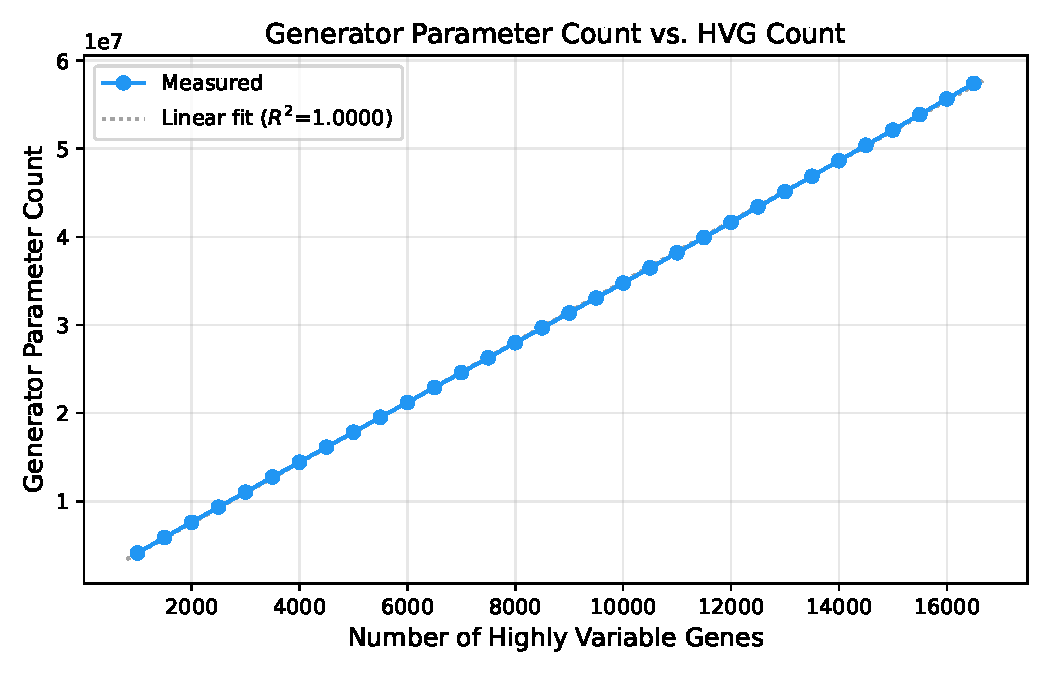
\includegraphics[width=0.95\textwidth]{gen_params_vs_hvg.pdf}
\caption{Generator parameter count as a function of the number of highly variable genes, fitted with $y = 3424.1 \cdot x + 670033$ ($R^2 = 1.0000$).}
\label{fig:gen-params}
\end{figure}

\begin{figure}[H]
\centering
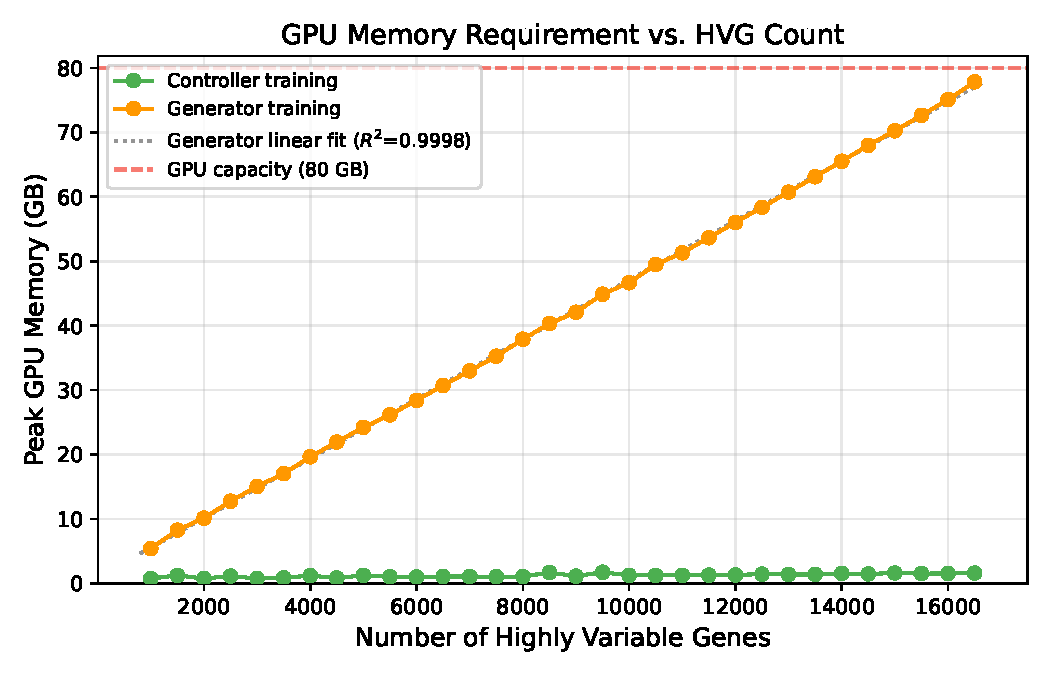
\includegraphics[width=0.95\textwidth]{gpu_mem_vs_hvg.pdf}
\caption{Peak GPU memory during controller and generator training as a function of HVG count. The red dashed line marks the GPU's total capacity (80\,GB = 81\,920\,MiB). The largest completed run approaches the capacity limit.}
\label{fig:gpu-mem}
\end{figure}

\begin{figure}[H]
\centering
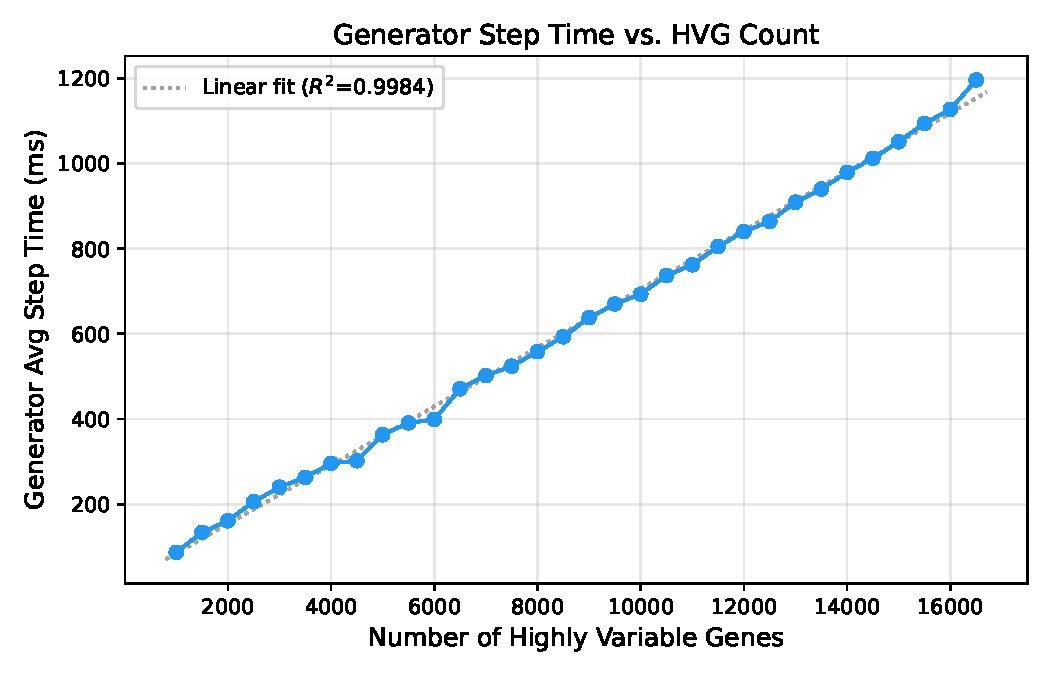
\includegraphics[width=0.95\textwidth]{gen_step_vs_hvg.pdf}
\caption{Causal generator average step time versus the number of highly variable genes. The dotted line is the linear fit used in the time equation above ($R^2 = 0.9984$).}
\label{fig:gen-step-hvg}
\end{figure}

\begin{figure}[H]
\centering
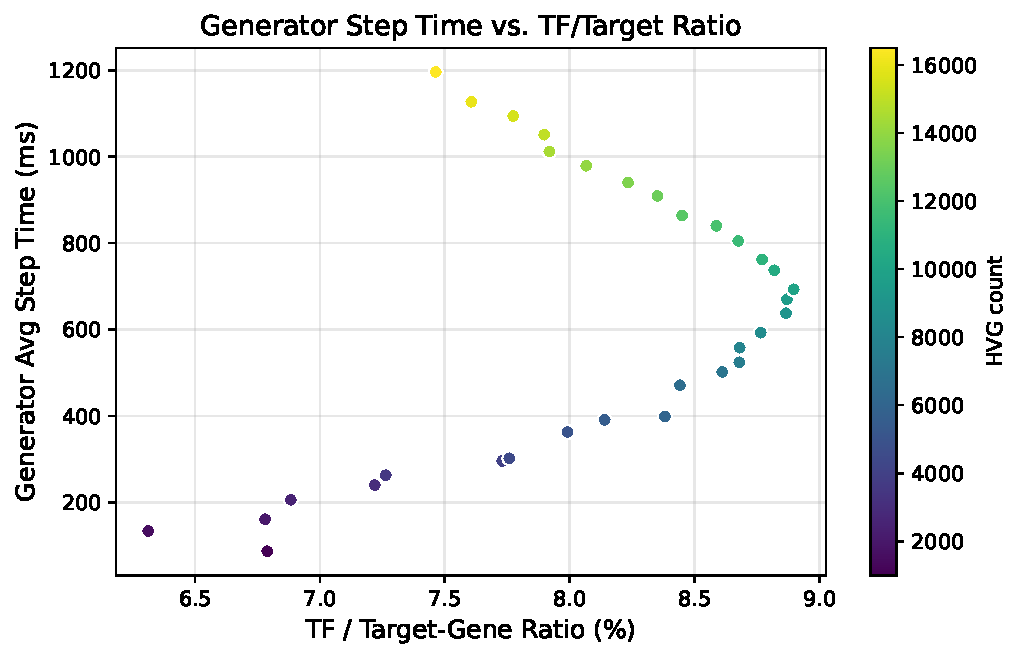
\includegraphics[width=0.95\textwidth]{gen_step_vs_ratio.pdf}
\caption{Causal generator average step time versus the TF/target-gene ratio. Point color indicates HVG count; the ratio is non-monotonic, peaking near 10{,}000 HVGs before declining at larger sizes.}
\label{fig:gen-step-ratio}
\end{figure}

\section{Notes}
\begin{itemize}
\item All runs use the same architecture: latent dim 128, generator layers 256--512--1024, critic layers 1024--512--256, labeler layers 2000--2000--2000, batch size 1024, 20 steps per phase.
\item The causal GAN trains in two phases: first the causal controller (a small GAN), then the full causal GAN (generator, critic, labeler, antilabeler). The controller uses minimal GPU memory; the generator phase dominates memory usage.
\item Included runs completed within the 80\,GB GPU budget. The excluded 17{,}000 HVG run hit CUDA out-of-memory during generator initialization.
\item Generator parameter counts scale linearly with HVG count ($R^2 = 1.0000$); generator step times also scale roughly linearly ($R^2 = 0.9984$, see Figure~\ref{fig:gen-step-hvg}).
\item The fitted generator requirements are $\widehat{M}_{\mathrm{gen}}(x) = 4.7268x + 927.7$ MiB and $\widehat{t}_{\mathrm{gen}}(x) = 0.06897x + 15.49$ ms/step ($R^2 = 0.9998$ and $R^2 = 0.9984$, respectively).
\item GPU memory values are in MiB as reported by \texttt{nvidia-smi}. The GPU total capacity is 81{,}920\,MiB (80\,GB).
\end{itemize}

\end{document}